\documentclass[a4paper,12pt]{report}
%\usepackage{biblatex}
%\usepackage[sectionbib]{chapterbib}%%% REFERENCE PAR CHARPITRE %%%
\usepackage[french,english]{babel}
\usepackage[nottoc]{tocbibind} 
\frenchbsetup{StandardLists=true}
\usepackage{enumitem}
%\usepackage[glenn]{fncychap}
\usepackage[T1]{fontenc}
\usepackage[utf8]{inputenc}
\usepackage{lmodern}
\usepackage{microtype}
\usepackage{graphicx}
\usepackage[font={small}]{caption}
%\usepackage[light, largesmallcaps]{kpfonts}%%%% LE FONT DE BASE DU TEXTE %%%%
\usepackage[top=2.5cm, bottom=2cm, left=3cm, right=2.5cm,
			headheight=15pt]{geometry}
					

\newcommand{\cia}{\begin{figure}[H]
\centering
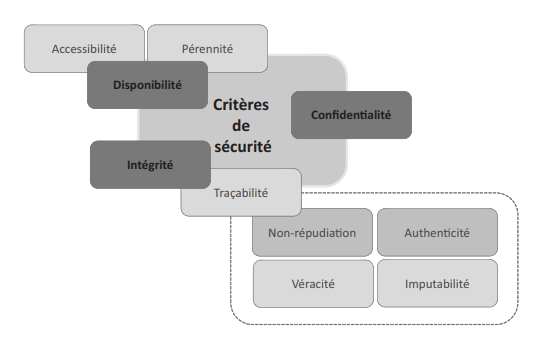
\includegraphics{images/CIA}
\caption{Critères de sécurité informatique \cite{ref4}}
\label{imagecia}
\end{figure}
}

\newcommand{\dl}{\begin{figure}[H]
\centering
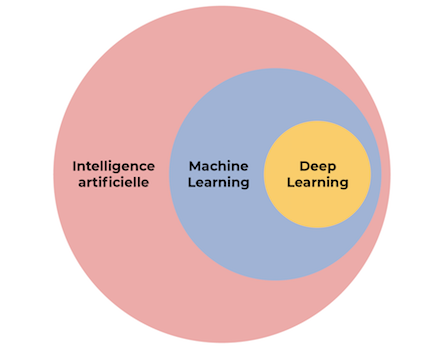
\includegraphics[height=5cm]{images/dl}
\caption{Position du Deep Learning dans l'IA \cite{refclassroom}}
\label{dl}
\end{figure}
}

\newcommand{\nslkdd}{\begin{figure}[H]
\centering
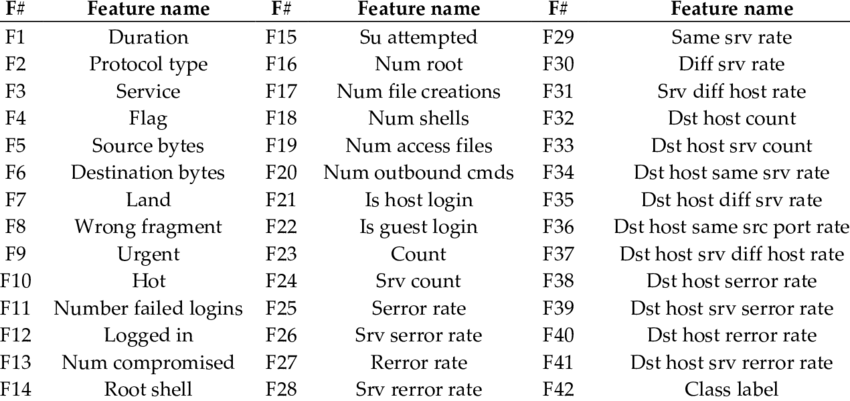
\includegraphics[width=\textwidth]{images/nslkdd}
\caption{Liste des caractéristiques de NSL-KDD. \cite{kdd}}
\label{nslkdd}
\end{figure}
}
\newcommand{\architecture}{\begin{figure}[H]
\centering
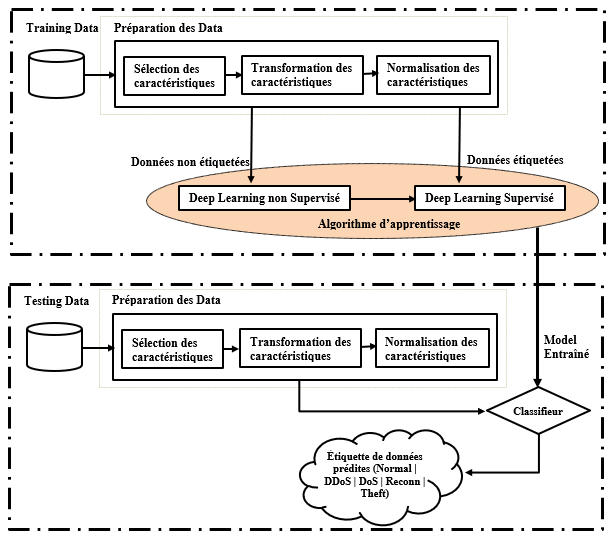
\includegraphics[width=\textwidth]{images/architecture}
\caption{L'architecture de notre approche }
\label{architecture}
\end{figure}
}
\newcommand{\modelAE}{\begin{figure}[H]
\centering
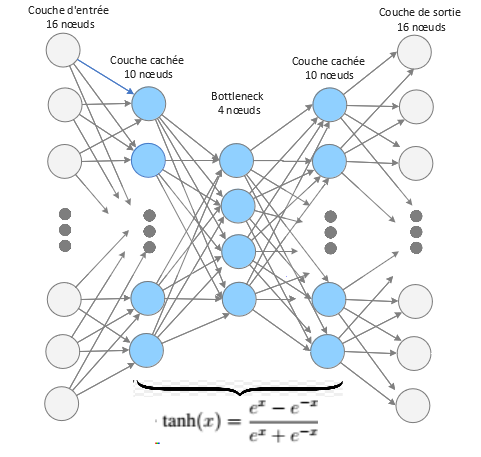
\includegraphics[width=\textwidth]{images/ModelAE}
\caption{Structure de l'AE}
\label{modelAE}
\end{figure}
}
\newcommand{\modelDNN}{\begin{figure}[H]
\centering
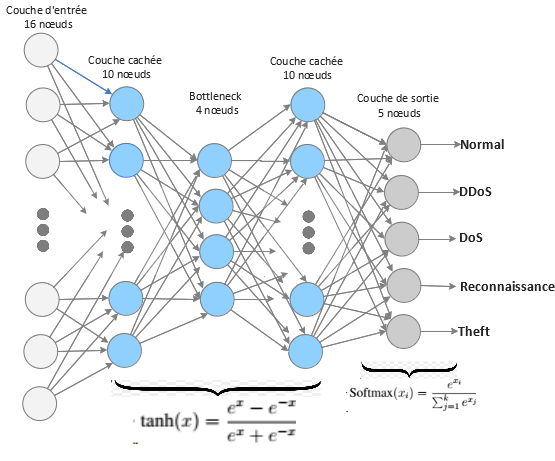
\includegraphics[width=\textwidth]{images/ModelDNN}
\caption{Structure du DNN}
\label{modelDNN}
\end{figure}
}
\newcommand{\iot}{\begin{figure}[H]
\centering
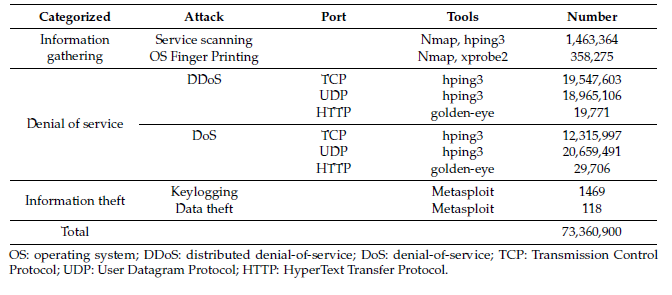
\includegraphics[width=\textwidth]{images/iot}
\caption{Résumé des attaques du Dataset Iot Botnet \cite{kdd}}
\label{nslkdd}
\end{figure}
}
%%%%%%%%%%%%%%%%%%%%%%%%%%%%%%%%%%%

\newcommand{\source}[1]{\caption*{ {#1}} 
}
%\source{\cite{ref4}}

\newcommand{\imageAPS}{\begin{figure}[!h]
\centering
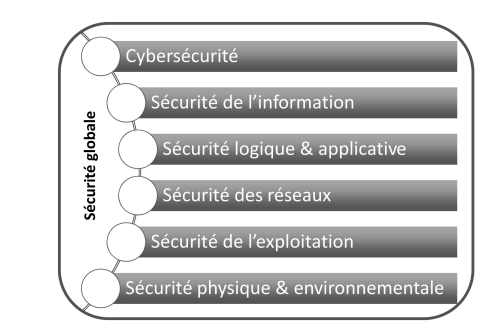
\includegraphics{images/applicationsécurité}
\caption{Application de sécurité informatique \cite{ref4}}
\label{imagecia}
\end{figure}
}

\newcommand{\imgMiM}{\begin{figure}[H]
\centering
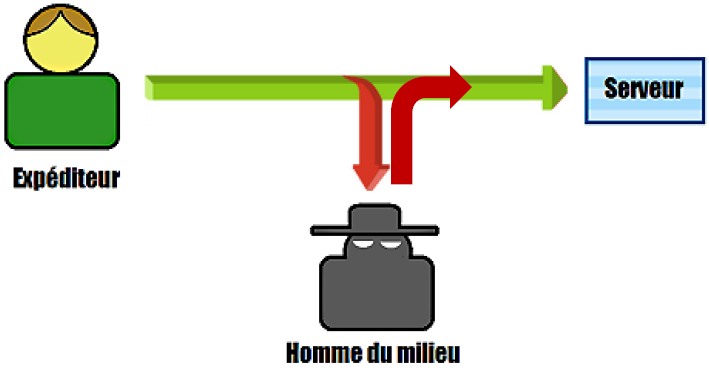
\includegraphics[width=\textwidth]{images/MiM}
\caption{main-in-the-middle}
\label{imagMiM}
\end{figure}
}
\newcommand{\typedl}{\begin{figure}[H]
\centering
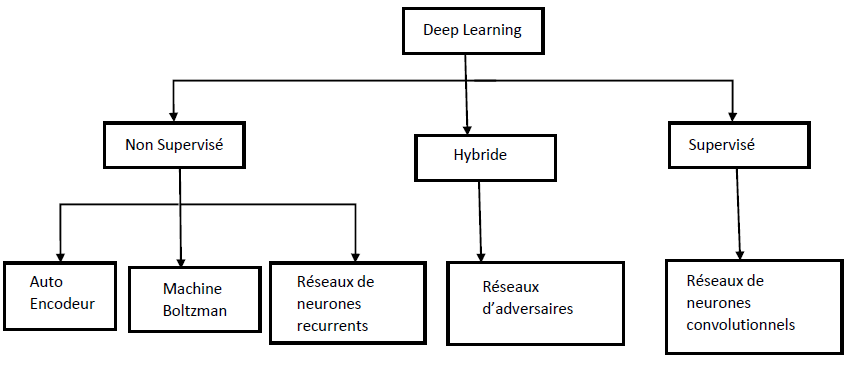
\includegraphics[width=\textwidth]{images/typedl}
\caption{classification des modèles de deep learning}
\label{typedl}
\end{figure}
}

\newcommand{\cnn}{\begin{figure}[H]
\centering
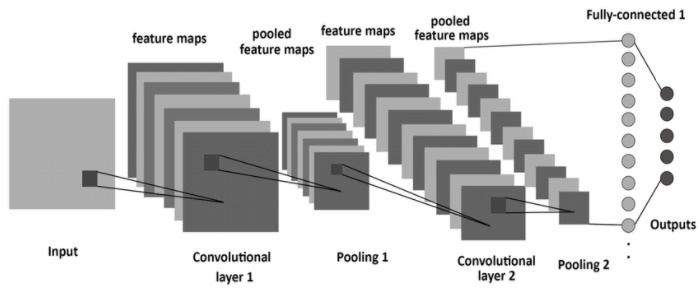
\includegraphics[width=\textwidth]{images/cnn}
\caption{Architecture classique d’un réseau de neurones convolutif \cite{cnn}}
\label{cnn}
\end{figure}
}

\newcommand{\autoencodeur}{\begin{figure}[H]
\centering
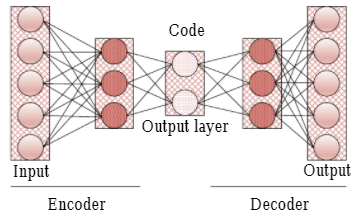
\includegraphics[width=\textwidth]{images/autoencodeur}
\caption{Architecture Auto Encodeur\cite{autoencodeur}}
\label{autoencodeur}
\end{figure}
}

\newcommand{\perceptron}{\begin{figure}[!h]
\centering
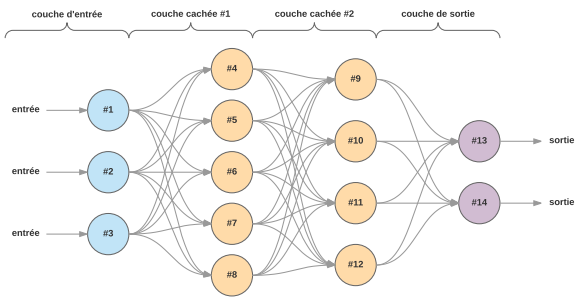
\includegraphics[width=\textwidth]{images/perceptron}
\caption{Réseau de neurone profond (DNN)}
\label{perceptron}
\end{figure}
}

\newcommand{\graphe}{\begin{figure}[H]
\centering
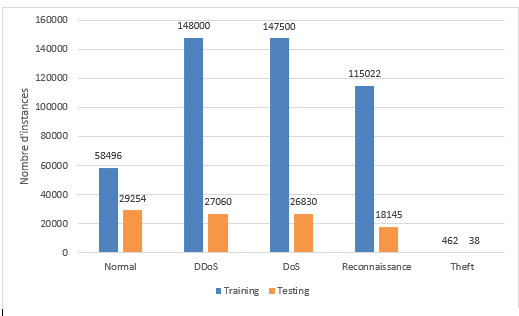
\includegraphics[width=\textwidth]{images/graphe}
\caption{Nombres d'éléments par types de datasets}
\label{graphe}
\end{figure}
}

\newcommand{\neurone}{\begin{figure}[H]
\centering
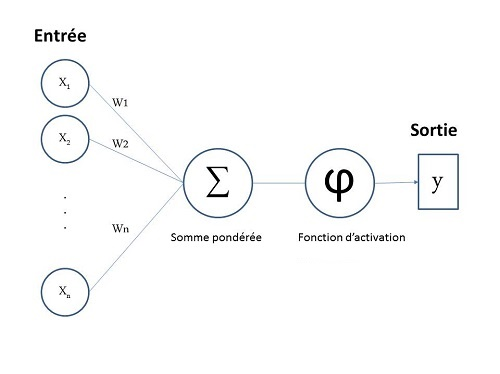
\includegraphics[height=7cm]{images/neuroneF}
\caption{Représentation d'un neurone formel}
\label{atnn}
\end{figure}
}

\newcommand{\cidf}{\begin{figure}[H]
\centering
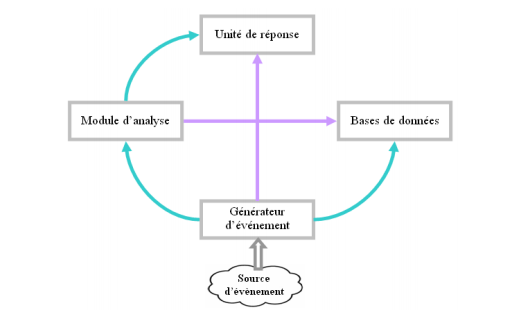
\includegraphics[width=\textwidth]{images/icef}
\caption{l’architecture CIDF \cite{zaidi}}
\label{imagMiM}
\end{figure}
}

\newcommand{\apprentissage}{\begin{figure}[H]
\centering
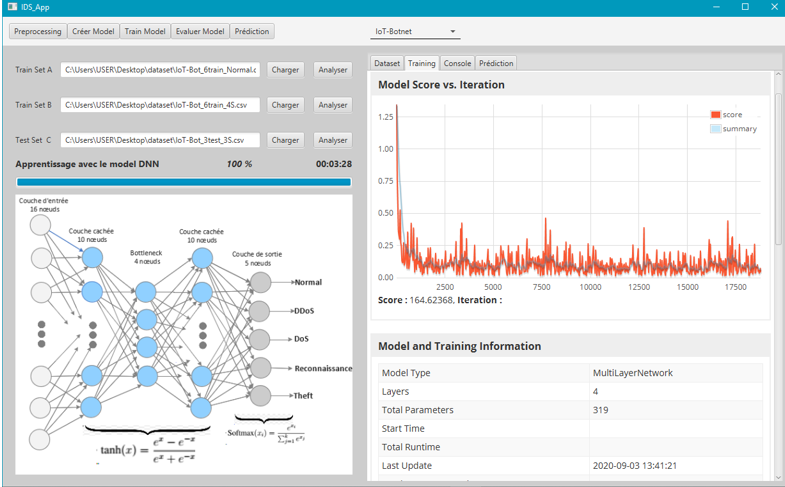
\includegraphics[width=\textwidth]{images/apprentissage}
\caption{Entrainement du modèle DNN}
\label{apprentisage}
\end{figure}
}

\newcommand{\prediction}{\begin{figure}[H]
\centering
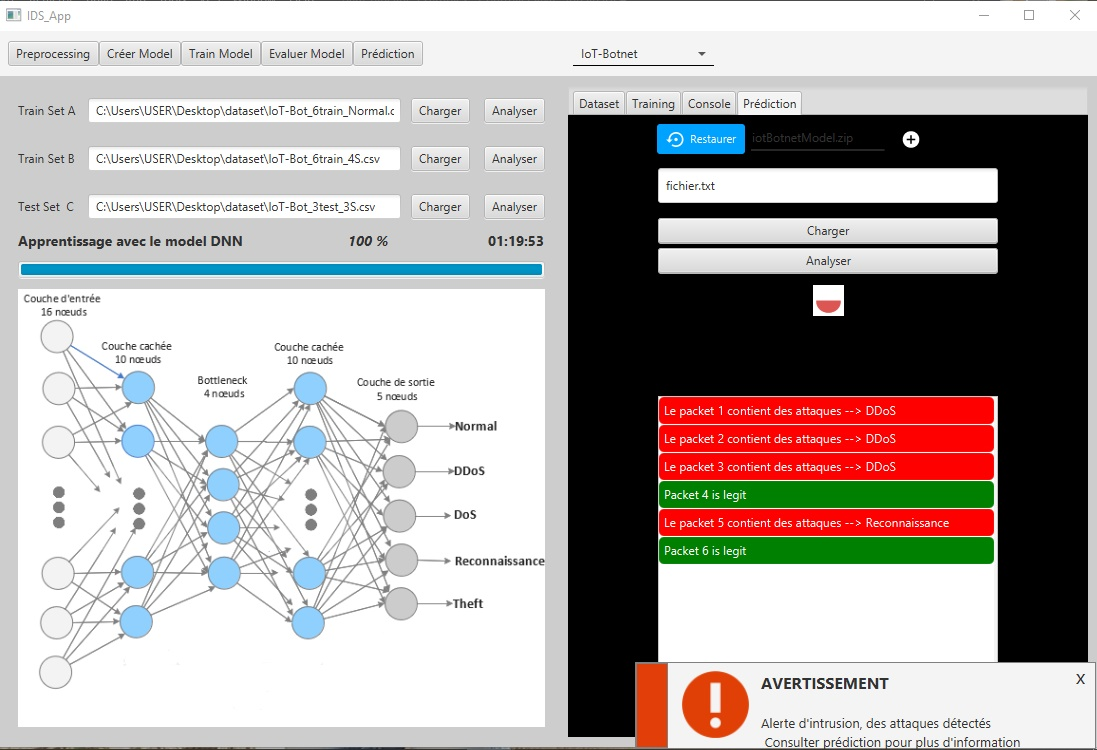
\includegraphics[width=\textwidth]{images/predi}
\caption{prédiction d'attaques}
\label{apprentisage}
\end{figure}
}

\newcommand{\data}{\begin{figure}[H]
\centering
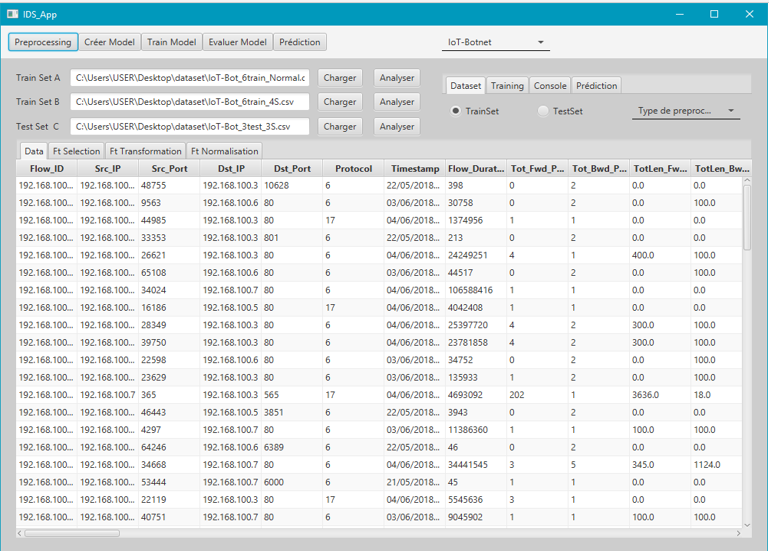
\includegraphics[width=\textwidth]{images/data}
\caption{structure du dataset}
\label{data}
\end{figure}
}

\newcommand{\analyse}{\begin{figure}[H]
\centering
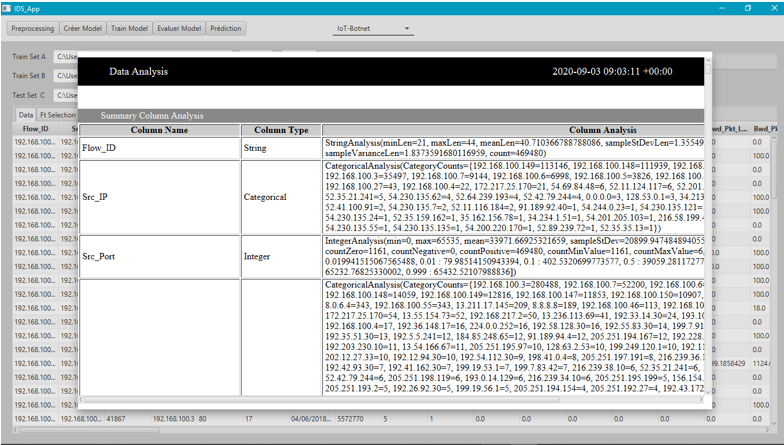
\includegraphics[width=\textwidth]{images/dataanalyse}
\caption{Analyse des données}
\label{data}
\end{figure}
}

\newcommand{\evaluation}{\begin{figure}[H]
\centering
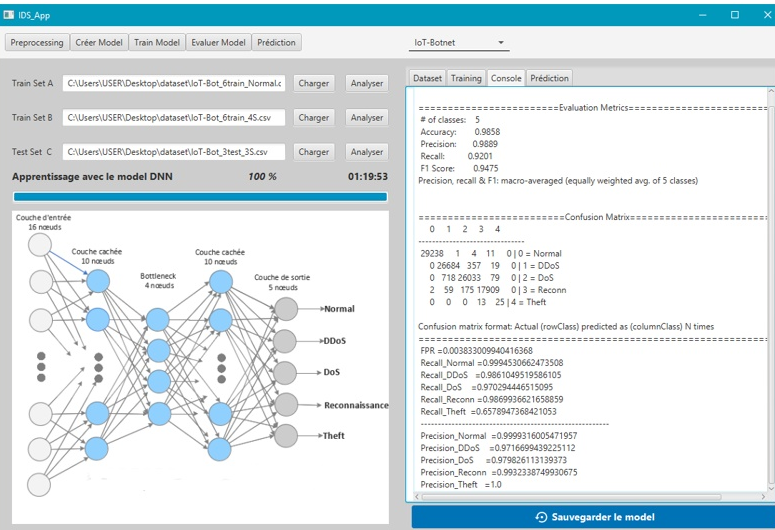
\includegraphics[width=\textwidth]{images/evaluation}
\caption{Evaluation du modèle}
\label{apprentisage}
\end{figure}
}
\newcommand{\idwg}{\begin{figure}[H]
\centering
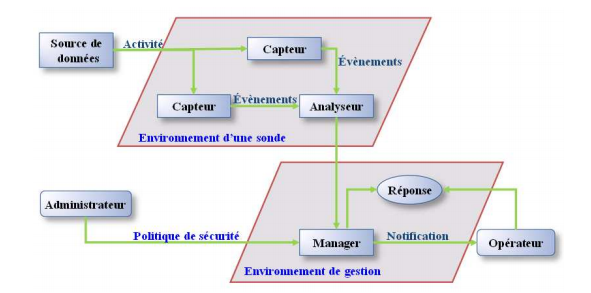
\includegraphics[width=\textwidth]{images/IDWG}
\caption{L’architecture IDWG \cite{zaidi}}
\label{idwg}
\end{figure}
}
\newcommand{\typeids}{\begin{figure}[H]
\centering
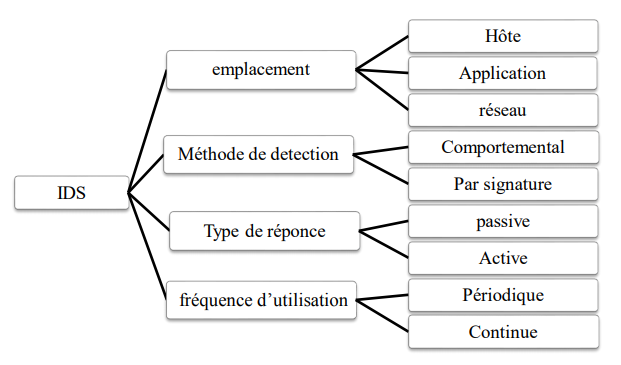
\includegraphics[width=\textwidth]{images/ids}
\caption{Classification des différents types d'IDS  \cite{reftypeids}}
\label{ids}
\end{figure}
}
\newcommand{\hids}{\begin{figure}[H]
\centering
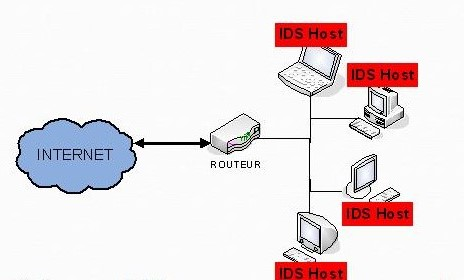
\includegraphics[width=\textwidth,height=10cm]{images/HIDS}
\caption{La détection d'intrusion basée sur l'hôte \cite{refphototypids}}
\label{hids}
\end{figure}
}
\newcommand{\nids}{\begin{figure}[H]
\centering
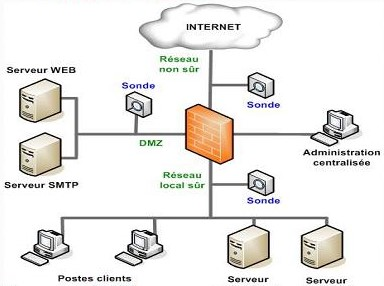
\includegraphics[width=\textwidth,height=10cm]{images/NIDS}
\caption{La Détection d'Intrusion Réseau (NIDS) \cite{refphototypids}}
\label{nids}
\end{figure}
}

\newcommand{\authenti}{\begin{figure}[H]
\centering
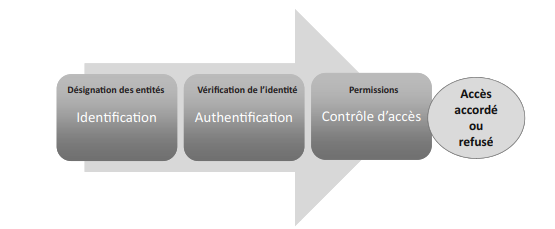
\includegraphics{images/authentification}
\caption{Accès à une ressource \cite{ref4}}
\label{Authentification}
\end{figure}
}

\newcommand{\ransom}{\begin{figure}[H]
\centering
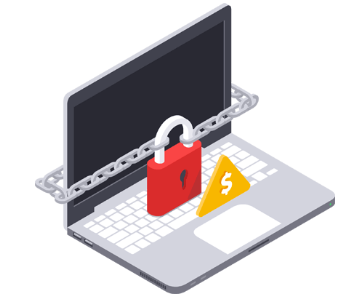
\includegraphics{images/ransomware}
\caption{Ransomware}
\label{ransomware}
\end{figure}
}


\newcommand{\logoucd}{\begin{figure}[!h]
\centering

\includegraphics[width=0.2\linewidth]{Images/uc2}
\label{logo}
\end{figure}
}
\newcommand{\pagedegarde}{
\begin{titlepage}
\newgeometry{top=1.5cm, bottom=1.5cm, left=2cm, right=1cm}
\AddToShipoutPicture*{\EtiquetteThese}
\begin{center}
\begin{minipage}{1\textwidth}
	\begin{center}
		\large\ministere{}
	\end{center}				
\end{minipage}
\vspace{0.9mm}
\logoucd\\
\Huge{\emph{{{\it {Mémoire de fin d'études}}}}}\\
\normalsize
\begin{center}
En vue de l'obtention du Diplôme de\\ 
 \huge{\textbf{MASTER EN INFORMATIQUE}}
\end{center}
\large{\textbf{Option }: Réseaux et Systèmes Distribués}

\vspace{1cm}
\Huge\textbf{Thème }
\noindent\rule{\textwidth}{0.9mm}
%\noindent\color{blueforest}\rule{\textwidth}{0.1mm}
\Large{\textbf{Approche résiliente pour l'identif{\kern0pt}ication et la détection des attaques DDoS dans les réseaux IoT}}
%\noindent\color{blueforest}\rule{\textwidth}{0.1mm}
\noindent\rule{\textwidth}{0.9mm}
\end{center}
\vspace{1.5cm}
\begin{tabular}{l r}
\hspace{1cm}\textbf{Présenté par :}&\hspace{5cm}\textbf{Sous la Direction de :}\\
\hspace{1cm}\textbf{\textcolor{blue}{Japhet DIARRA }}&\textbf{\textcolor{blue}{$M^{r}$ Amir DJENNA}}\\
\hspace{1cm}\textbf{\textcolor{blue}{ Mamadou DIARRA MAKADJI TB}}&\textbf{}
\end{tabular}
\begin{center}
\vspace{1.5cm}
\hspace{0.3cm}\textbf{\large{Devant le jury composé de : }}\\
\vspace{0.5cm}
\begin{tabular}{llll}
%\vspace{0.1cm}
\hspace{0.3cm}\textbf{\textbf{ Président : }} \hspace{0.8cm} $M^{r}$ \textbf{Abdellatif  HABES} \\
\vspace{0.1cm}
\hspace{0.3cm}\textbf{\textbf{Examinatrice : }} \hspace{0.2cm} $M_{me}$ \textbf{Houda  HAFI}
%\hspace{3.1cm} \hspace{0cm} $M^{elle}$ \textsl{XXXX} Xxxx \hspace{2.09cm} \textsl{ \emph{X, Université Constantine 02}}\\
\end{tabular}
\end{center}
\vspace{2cm}
\begin{center}
\textbf{Septembre 2020}
\end{center}
\end{titlepage}
\restoregeometry  
\nopagebreak
}
\newcommand{\firstpart}{\part{\'Etat de l'art}}
\newcommand{\secondpart}{\part{Contributions}}
\newcommand{\ministere}{R\'{e}publique  Alg\'{e}rienne D\'{e}mocratique et Populaire\\Ministère de  l'Enseignement Sup\'{e}rieur et de la Recherche Scientifique\\Université Constantine 2 – Abdelhamid Mehri \\Faculté des Nouvelles Technologies de l'Information et de la Communication (NTIC)\\ Département d’Informatique Fondamentale et ses Applications (IFA)}
\definecolor{blueforest}{RGB}{00,74,09}
\newcommand\EtiquetteThese{%
	\put(-10,10){%
		\parbox[t][\paperheight]{\paperwidth}{%
			\hfill
			\colorbox{blueforest}{		
				\begin{minipage}[b]{3em}
				\vspace{0.1cm}
					\centering\Huge\textcolor{white}{\textbf{M}\\\textbf{A}\\\textbf{S}\\\textbf{T}\\\textbf{E}\\\textbf{ R}}
					\vspace{0.2cm}
				\end{minipage}
			}
		}
	}
}




%%%%%%%%%%%%%%%%%%%HEADER FOOTER%%%%%%%%%%%%%%%%%%%%%%%%%%%%%%%%%%%
\usepackage{fancyhdr}
\fancyhf{}
\renewcommand{\headrulewidth}{2pt}
\renewcommand{\footrulewidth}{1pt}
\lhead{\leftmark}
\cfoot{\thepage}
\pagestyle{fancy}			
\usepackage{titlesec}
\titleformat{\chapter}[display]
  {\bfseries\Large}
  {\filright\MakeUppercase{\chaptertitlename} \Huge\thechapter}
  {1ex}
  {\titlerule\vspace{0.5ex}\center}
  [\vspace{1ex}\titlerule]
\usepackage[french]{minitoc}%%%% Tables de matière par chapitre  
\usepackage[colorlinks=true,linkcolor=blue, citecolor=blue]{hyperref}

\dominitoc
\setcounter{minitocdepth}{1}
\setcounter{tocdepth}{3}
\setcounter{secnumdepth}{3} 
\begin{document}
\fontfamily{ptm}\selectfont


\addcontentsline{toc}{part}{Introduction Générale}
\markboth{\textbf{INTRODUCTION G\'EN\'ERALE}}{}
\chapter*{Introduction générale}
\parindent=0.2cm	
Les progrès fulgurants des Technologies de l’Information et de la Communication(\textbf{TIC}) et le bésoin de faire collaborer des objets ont conduit à un concept moderne qui est « Internet of Things \footnote{Nous utilisons tout le long de notre mémoire l’abréviation IoT pour « Internet of Things », qui se traduit en français par l’Internet des objets}» (\textbf{IoT}). L'IoT nous offre une nouvelle opportunité de croissance nous permettant délimiter la perte de temps, de ressource, améliorant ainsi nos vie quotidiennes.De nos jours, il existe de nombreuses plateformes et applications pour l’IoT conduisant à fournir de nouveaux services et automatiser de nombreux processus dans l'industrie(smart industry), la santé(smart health), le ménage, les transports(smart transport) et de nombreux autres secteurs etc.\\

Il existe plusieurs définitions sur le concept de l’IoT, mais nous adoptons celle proposée par Weill et Souissi qui ont défini l’IoT comme « une extension de l'Internet actuel envers tout objet pouvant communiquer de manière directe ou indirecte avec des équipements électroniques eux-mêmes connectés, à l'Internet. Cette nouvelle dimension de l'Internet s'accompagne avec de forts enjeux technologiques, économiques et sociaux tout en assurant la protection des données des utilisateurs » \cite{refdiot}. Quasiment n'importe quel appareil doté d'un bouton marche/arrêt peut se connecter à l'Internet aujourd'hui, intégrant ainsi la catégorie des objets de l'IoT \cite{ciscorefiot}\\ 
En ce qui concerne l'IoT, Les objets connectés peuvent être des objets  physiques ou virtuelles (smartphones, ordinateurs, data centers, réseaux Wi-Fi, réseaux cellulaires, puces RFID , capteurs, équipement ménager, montres, serrures, véhicules, drones, etc ) pouvant être identifiés et intégrés dans la communication des réseaux.\\
D'après la plateforme statisca \cite{refstatic} aujourd'hui le nombre d'objets connectés est estimé à \textbf{30.73 milliards} d'objets connectés dans le monde et ce nombre atteindrait les \textbf{75.44 milliards } d'objets connectés en 2025.\\

Cependant assurer la confidentialité, la disponibilité et l'intégrité des objets connectés ainsi que les données qui y transitent sont les principales préoccupations concernant l'adoption de ce nouveau concept l'IoT. Une fois que les appareils sont connectés à Internet, ils deviennent vulnérables à d'éventuelles d'attaques informatiques. l'IoT étant la prochaine génération  d'Internet \cite{cisco} avec de plus en plus d'objets connectés allant des villes connectés aux vaches connectées. Dans ce réseau les objets connectés s’échangent des informations pour répondre à un but bien défini. Cette collaboration des objets ouvre des portes d’attaques aux hackers qui effectuent des attaques de plus en plus sophistiquées.\\

Selon 451 Research \cite{ref451rec} beaucoup d'entreprises sont toujours retissant dans l'adoption de l'IoT à cause sa gestion de la sécurité de ce nouveau qui est encore en état embryonnaire, mais 55\% des entreprises qui ont adoptées l'IoT classent la gestion de la sécurité IoT comme leur priorité absolue lors des déploiements de projets IoT au sein de leurs organisations. Les systèmes vulnérables des objets connectés  peuvent être compromis de n’importe où et utilisés pour cibler n’importe qui raison pour laquelle la sécurité IoT est une préoccupation mondiale.\\

Les objets connectés font faces à plus types de menaces. ces types de menaces sont classées en quatre(4) types \cite{refinfosec} : 
\begin{itemize}
\item \textbf{Déni de Service :} Cette menace vise la disponibilité d'un service ou d'une ressource en la saturant de requête indésirable empêchant ainsi ses utilisateurs légitimes de l'utiliser. cette indisponibilité du service ou d'une ressource est mise en œuvre avec par l'attaque de types DDoS. C'est probablement l'une des ménaces les plus courantes et les plus dangereuses . 
\item \textbf{les logiciels malveillants} Un auteur de malware conçoit spécifiquement ses codes pour compromettre les architectures utilisées par les appareils IoT. Un code malveillant pourrait être utilisé pour infecter les ordinateurs utilisés pour contrôler un réseau d'appareils intelligents ou pour compromettre le logiciel qui y est exécuté. Dans ce deuxième scénario, les attaquants peuvent exploiter la présence d'une faille dans le micrologiciel exécuté sur les appareils et exécuter leur code arbitraire, transformant les composants IoT en utilisation non planifiée \cite{refinfosec}
\item \textbf{Violation de données (Data Breaches) : } C'est une menace visant l'intégrité et la confidentialité des données. les attaquants peuvent utiliser des attaques de type homme du milieu pour intercepter les communications des objets connectés.  
\item \textbf{Affaiblissement des périmètres : } Les appareils de l'Internet des objets ne sont généralement pas conçus pour la sécurité. Bien qu'il s'agisse d'appareils connectés à Internet, la majorité des appareils ne disposent pas de mécanismes de sécurité réseau. Prenons, par exemple, un compteur intelligent. Si l'attaquant est en mesure de le compromettre, il pourrait avoir accès à notre réseau domestique, nous espionner ou causer des dommages physiques à notre environnement domestique. Le problème est tout aussi grave si nous considérons l'utilisation d'appareils IoT dans n'importe quelle industrie.\cite{refinfosec}
\end{itemize}

Nous nous focaliseront dans ce mémoire sur la menace « déni de service \footnote{Nous utilisons tout le long de notre mémoire l’abréviation DoS pour « Denial of Service », qui se traduit en français par déni de Service}( \textbf{DoS})», notamment l'attaque par « Déni de Service Distribué\footnote{Nous utilisons tout le long de notre mémoire l’abréviation DDoS pour « Distributed Denial of Service », qui se traduit en français par déni de service distribué}( \textbf{DDoS})». une attaque par déni de service est une attaque qui empêche l'accès à une ressource ou à un service internet. Elle obtenue en saturant avec des centaines de milliers voire des millions de connexions(requêtes) un serveur ou un objet connecté jusqu'à le bloquer.\\

\textbf{À titre d'exemple : } \begin{itemize}
\item En 2007 l'Estonie \cite{refestonie} a été victime de la première plus grande attaque DDoS de l'histoire. l'attaque visait le système informatique du pays notamment ses sites gouvernementaux, ses banques et ses médias créant la panique et déclenchant de vaste d'émeute au sein de la population et force de l'ordre. 
\item En octobre 2016 \cite{refddos} Dyn un important fournisseur de service de noms de domaine a été victime d'une vague d'attaque par déni de service distribuée. l'attaque était orchestrée à l'aide d'un logiciel malveillant appelé Mirai, les pirates se sont servis de ce programme pour créer un énorme botnet\footnote{ un botnet est un réseau d'objet connectés contrôlé par un hacker } de 100000 objets connectés pour lanceur leur attaque. L'attaque a été extrêmement perturbatrice et a fait tomber les sites Web de plus de 80 de ses clients, notamment Amazon, Netflix, Airbnb, Spotify, Twitter, PayPal et Reddit. Les dommages causés par cette attaque auraient coûté 110 millions de dollars ainsi que la dégradation de la réputation du fournisseur.
\item En 2018 github, une plateforme de développement à son tour était visée d'attaque DDoS qui a été. l'attaque a été maitrisée 10 min après \cite{refddos} grâce à la présence système de protection d'attaque DDoS dans la plateforme.  
\end{itemize}
Nous proposons dans ce mémoire \textit{la mise en place d'un système de détection d'intrusion dans le réseau IoT contre les attaques de types DDoS.} afin d'assurer la disponibilité d'un service ou d'un objet connecté dans le réseau IoT.\\  

Notre choix du DDoS s'explique du fait que le DDoS utilise les objets connectées non sécurisés pour sa mise œuvre et du fait qu'elle est actuellement considérée comme l'attaque la plus dangereuse visant l'IoT \cite{8355541} \cite{inproceedings}.\\

Ce document est organisée en 2 parties :

\begin{description}
\item[\textbf{La première partie :}] présente l'état de l'art sur les différents domaines entrant en jeu dans le cadre de ce mémoire à savoir la sécurité informatique et la cybersécurité, l'attaque par déni de service distribué (\textbf{DDoS}), l'Internet des objets(\textbf{l'IoT})  --------- A COMPLETER PAR LA SUITE --------
\item[\textbf{La seconde partie : }]----------- PRESENTERA LES CONTRIBUTIONS APPORTEES-------- 
\end{description}

%%%%%%%%%% REFERENCES BIBLIOGRAPHIQUES %%%%%%%%%
\clearpage			
\bibliographystyle{apalike}
\markboth{Bibliographie}{}
\bibliography{biblo}

\end{document}
